% !TeX root = ../libro.tex
% !TeX encoding = utf8

\chapter{Demostraciones adicionales}\label{ap:demostraciones-adicionales}

% ===================+
\begin{proposicion}\label{prop:ap-mtm}
Toda máquina de Turing multicinta puede ser simulada por una máquina de Turing de una sola cinta.
\end{proposicion}
\begin{proof}
Sea $M=(Q, A, B, \delta, q_0, \Vtextvisiblespace\:, F)$ una máquina de Turing con $k$ cintas. Definiremos la máquina $\widetilde{M}=(\widetilde{Q}, A, \widetilde{B}, \widetilde{\delta}, q_0, [\Vtextvisiblespace^k], F)$. Para ello, definimos en primer lugar $\widecheck{B}$ como:
$$
    \widecheck{B} = \{\widecheck{b} : b \in B\}
$$
Para definir $\widetilde{B}$, observemos que un símbolo de un alfabeto no tiene por qué ser únicamente un carácter. Para representar un único símbolo, lo rodearemos de corchetes ($[\:]$). Por tanto, el siguiente alfabeto tiene sentido:
$$
    \widetilde{B} = \{[u_1\:u_2\:...\:u_k]:u_i\in B\cup\widecheck{B}\}\cup\{\#\}
$$
En $\widetilde{B}$ insertamos, además de los símbolos que hemos comentado, un símbolo delimitador $\#$.

El conjunto de estados $\widetilde{Q}$ lo hacemos más amplio que $Q$. Para ello, numeraremos todos los estados de $Q$:
$$
    Q=\{q_0,q_1,...,q_m\}
$$
Y definimos el nuevo conjunto de estados como:
$$
    \widetilde{Q}=Q\cup\left(\bigcup_{i=0}^m\bigcup_{j=1}^k\left\{\widetilde{q}_{i,j},\:\widetilde{q}_{i,j}^{(R)},\:\widetilde{q}_{i,j}^{(I)},\:\widetilde{q}_{i,j}^{(Is)},\:\widetilde{q}_{i,j}^{(D)},\:\widetilde{q}_{i,j}^{(Ds)}\right\}\right)
$$
Definimos como configuración inicial de la máquina con entrada $u=u_1\:u_2\:...\:u_n\in A^*$ a:\footnote{Siempre es posible cambiar la posición de la configuración inicial de una máquina de Turing, ejecutando las transiciones necesarias.}
$$
    q_0\;:\;\fbox{\#}\:[\widecheck{u_1}\:\underbrace{\widecheck{\Vtextvisiblespace} \:... \:\widecheck{\Vtextvisiblespace}}_{k-1)}]\:[u_2\:\underbrace{{\Vtextvisiblespace} \:... \:{\Vtextvisiblespace}}_{k-1)}]\:...\:[u_n\:\underbrace{{\Vtextvisiblespace} \:... \:{\Vtextvisiblespace}}_{k-1)}]\:\#
$$
Describiremos $\widetilde{\delta}$ poco a poco. En primer lugar, queremos partir del mismo estado que la máquina multicinta (esto nos permitirá que el lenguaje aceptado sea el mismo, como veremos más adelante). En el momento en el que la máquina se encuentre en este estado, nos movemos a la derecha y comenzaremos a buscar la posición en la cinta del primer cabezal. Usaremos el estado $\widetilde{q}_{i,j}$ para buscar el cabezal $j$-ésimo, estando la máquina multicinta en el estado $q_i$. Añadimos para hacer esto las siguientes transiciones:
\begin{equation}
    \widetilde{\delta}(q_i, \#) = (\widetilde{q}_{i,1}, \#, D)\;\;\text{ para cada }\;\;i=0,1,...,m
\end{equation}
Para buscar el cabezal $j$-ésimo, estando la máquina multicinta en el estado $q_i$, nos iremos moviendo a la derecha mientras que no hayamos encontrado un carácter de $\widecheck{B}$ en la posición $j$-ésima. Para ello, añadimos para cada $i=0,1,...,m$ y $j=1,2,...,k$:
\begin{equation}
    \widetilde{\delta}(\widetilde{q}_{i,j}, [ w_1\:w_2\:...\:w_l\:...\:w_k]) = (\widetilde{q}_{i,j}, [ w_1\:w_2\:...\:w_l\:...\:w_k], D)\;\;\text{ con }\;\;w_j\in B, w_l \in B\cup\widecheck{B} \text{ para } l \neq j
\end{equation}
Nótese que, de forma explícita, hacemos que el símbolo $w_j$ no pueda estar en $\widecheck{B}$ (de aquí en adelante, si no explicitamos, será $w_l\in B\cup\widecheck{B}$ para cada $l=0,1,...,k$). Esto es para continuar moviéndonos a la derecha hasta encontrar un carácter con cabezal en la posición $j$-ésima de cada símbolo.

Ahora estamos en condiciones de incluir las transiciones de $\delta$ en $\widetilde{\delta}$. Sea una transición de $\delta$:
$$
    \delta(q_i, b_1, b_2, ..., b_k) = (q_j, c_1, M_1, c_2, M_2, ..., c_k, M_k)
$$
Para cada una de estas transiciones, deberemos insertar reglas en $\widetilde{\delta}$. Estas transiciones dependerán de cómo se mueva el cabezal, ya que si lo hace a la derecha o a la izquierda hasta toparse con el delimitador $\#$, deberemos extender la cinta de $\widetilde{M}$ con un símbolo blanco de $\widetilde{M}$ (que es $[\Vtextvisiblespace^k]$), y desplazar el delimitador $\#$ una posición. Dada la transición anterior, y para cada $l=1, 2, ..., k$:
\begin{itemize}
    \item Si $M_l=D$, insertamos varias transiciones. En primer lugar, la transición correspondiente a sustituir el símbolo en el que se encuentra el cabezal, $b_l$, por el correspondiente, $c_l$:
    \begin{equation}
        \widetilde{\delta}(\widetilde{q}_{i,l}, [w_1\:w_2\:...\:w_{l-1}\:\widecheck{b_l}\:w_{l+1}\:...\:w_k]) = (\widetilde{q}_{i,l}^{(D)}, [w_1\:w_2\:...\:w_{l-1}\:c_l\:w_{l+1}\:...\:w_k], D)
    \end{equation}
    A continuación simulamos que el cabezal $l$-ésimo se mueve a la derecha. En caso de que no hayamos alcanzado el separador $\#$, la transición es directa, simplemente indicamos que el cabezal está en la posición determinada, y volvemos al primer delimitador $\#$ mediante el estado $^{(R)}$ (que veremos más adelante):
    \begin{equation}
        \widetilde{\delta}(\widetilde{q}_{i,l}^{(D)}, [w_1\:w_2\:...\:w_{l-1}\:w_l\:w_{l+1}\:...\:w_k]) = (\widetilde{q}_{i,l}^{(R)}, [w_1\:w_2\:...\:w_{l-1}\:\widecheck{w_l}\:w_{l+1}\:...\:w_k], I)
    \end{equation}
    En caso de que nos topemos con el delimitador $\#$, iniciaremos una ``subrutina'' indicada con los estados $^{(Ds)}$, en el que añadiremos un símbolo blanco y moveremos el delimitador a la derecha, siguiendo al estado $^{(R)}$:
    \begin{align}
        \widetilde{\delta}(\widetilde{q}_{i,l}^{(D)}, \#) &= (\widetilde{q}_{i,l}^{(Ds)}, [\underbrace{{\Vtextvisiblespace} \:... \:{\Vtextvisiblespace}}_{l-1)}\:\widecheck{\Vtextvisiblespace}\:\underbrace{{\Vtextvisiblespace} \:... \:{\Vtextvisiblespace}}_{k-l)}], D)\\
        \widetilde{\delta}(\widetilde{q}_{i,l}^{(Ds)}, [\Vtextvisiblespace^k]) &= (\widetilde{q}_{i,l}^{(R)}, \#, I)\\
    \end{align}
    \item Si $M_l=I$, añadimos de forma análoga las transiciones:
    \begin{align}
        \widetilde{\delta}(\widetilde{q}_{i,l}, [w_1\:w_2\:...\:w_{l-1}\:\widecheck{b_l}\:w_{l+1}\:...\:w_k]) &= (\widetilde{q}_{i,l}^{(I)}, [w_1\:w_2\:...\:w_{l-1}\:c_l\:w_{l+1}\:...\:w_k], I)\\
        \widetilde{\delta}(\widetilde{q}_{i,l}^{(I)}, [w_1\:w_2\:...\:w_{l-1}\:w_l\:w_{l+1}\:...\:w_k]) &= (\widetilde{q}_{i,l}^{(R)}, [w_1\:w_2\:...\:w_{l-1}\:\widecheck{w_l}\:w_{l+1}\:...\:w_k], I)\\
        \widetilde{\delta}(\widetilde{q}_{i,l}^{(I)}, \#) &= (\widetilde{q}_{i,l}^{(Is)}, [\underbrace{{\Vtextvisiblespace} \:... \:{\Vtextvisiblespace}}_{l-1)}\:\widecheck{\Vtextvisiblespace}\:\underbrace{{\Vtextvisiblespace} \:... \:{\Vtextvisiblespace}}_{k-l)}], I)\\
        \widetilde{\delta}(\widetilde{q}_{i,l}^{(Is)}, [\Vtextvisiblespace^k]) &= (\widetilde{q}_{i,l}^{(R)}, \#, D)\\
    \end{align}
    \item Si $M_l=S$, la transición es más inmediata, dado que no debemos mover el cabezal, simplemente reemplazar el símbolo y cambiar a $^{(R)}$:
    \begin{align}
        \widetilde{\delta}(\widetilde{q}_{i,l}, [w_1\:w_2\:...\:w_{l-1}\:\widecheck{b_l}\:w_{l+1}\:...\:w_k]) &= (\widetilde{q}_{i,l}^{(R)}, [w_1\:w_2\:...\:w_{l-1}\:\widecheck{c_l}\:w_{l+1}\:...\:w_k], I)
    \end{align}
\end{itemize}
Ahora, nos queda una forma de cambiar la cinta que estamos analizando. Comenzaremos añadiendo para ello un estado de retorno, que posiciona el cabezal en el primer delimitador $\#$. Para cada $i=0,1,...,m$ y $j=1,2,...,k$ añadimos las transiciones:
\begin{equation}
    \widetilde{\delta}(\widetilde{q}_{i,j}^{(R)}, [w_1\:w_2\:...\:w_l\:...\:w_k]) = (\widetilde{q}_{i,j}^{(R)}, [w_1\:w_2\:...\:w_l\:...\:w_k], I)
\end{equation}
Para leer la cinta siguiente, simplemente añadimos estas transiciones para cada $i=0,1,...,m$ y $j=1,2,...,k-1$:
\begin{equation}
    \widetilde{\delta}(\widetilde{q}_{i,j}^{(R)}, \#) = (\widetilde{q}_{i,j+1}^{(R)}, \#, D)
\end{equation}
Si ya hemos leído la última cinta, cambiamos el estado a uno de los de $Q$ de acuerdo a la función de transición. De nuevo revisitamos $\delta$. Para cada transición:
$$
    \delta(q_i, b_1, b_2, ..., b_k) = (q_j, c_1, M_1, c_2, M_2, ..., c_k, M_k)
$$
añadimos la transición de cambio de estado:
\begin{equation}
    \widetilde{\delta}(\widetilde{q}_{i,k}^{(R)}, \#) = (q_j, \#, S)
\end{equation}
Ya hemos definido todas las transiciones necesarias. Ahora, comprobaremos que la simulación es correcta, es decir, que $L(M)=L(\widetilde{M})$. En efecto, hemos construido una máquina $\widetilde{M}$ que ejecuta el mismo proceso de cálculo que $M$, y que además pasa por los mismos estados $Q$ de $M$ tras modificar la cinta. En otras palabras, la máquina $M$  Es precisamente por esto por lo que, en caso de la máquina parar, se encontrará en un estado $q\in Q$ (la hemos construido para que ocurra esto). De este modo, el lenguaje aceptado por ambas máquinas coincide, dado que usamos el mismo conjunto de estados finales $F$.
\end{proof}
% ===================+

\pagebreak

% ===================+
\begin{proposicion}\label{prop:f-s}
Para cada problema $F:X\longrightarrow Y$, existe un problema equivalente $\widehat{F}:S\longrightarrow S$.
\end{proposicion}
\begin{proof}
Si queremos resolver un problema de ordenador, deberemos codificar las entradas y las salidas mediante un formato que pueda entender. La idea es poder traducir un problema $F$ a otro problema $\widehat{F}$ de \emph{strings}, de modo que procese la misma función $F$ para entradas correctamente codificadas, y se devuelva \palabra{no} en caso de que la codificación de entrada sea incorrecta.

Para formalizar este concepto convenientemente, definiremos los conjuntos $X^\oslash = X \cup \{\oslash\}$ y $Y^\oslash = Y \cup \{\oslash\}$. A $\oslash$ lo llamaremos el \emph{elemento error}.

Expandiremos el problema $F$ para aceptar el elemento error como entrada, de modo que su solución sea el elemento error. Lo llamaremos $F^\oslash : X^\oslash \longrightarrow Y^\oslash$, definido como:
$$
    F^\oslash(x) = \begin{cases} 
      F(x), & \text{si} \;\;\; x \in X \\
      \oslash, & \text{si} \;\;\; x = \oslash 
   \end{cases}
$$
Sea $\mathcal{C}_X : S \longrightarrow X^\oslash$ la función que, para cada codificación en $S$, asigna la entrada de $X$ correspondiente. Si la codificación es inválida, asigna $\oslash$.

Sea $\mathcal{C}_Y^* : Y^\oslash \longrightarrow S$ la función que, para cada solución de $Y$, asigna la codificación en $S$ correspondiente. Para la solución error $\oslash$, asigna la codificación \palabra{no}. Del mismo modo que para las entradas, también podemos definir $\mathcal{C}_Y : S \longrightarrow Y^\oslash$, que para cada codificación de una solución en $S$, obtiene su solución en $Y$. Para codificaciones inválidas, asigna $\oslash$.

Ahora estamos en condiciones de definir $\widehat{F} = \mathcal{C}_Y^* \circ F^\oslash \circ \mathcal{C}_X$.
\begin{figure}[H]
\centering

\tikzset{every picture/.style={line width=0.75pt}} %set default line width to 0.75pt        

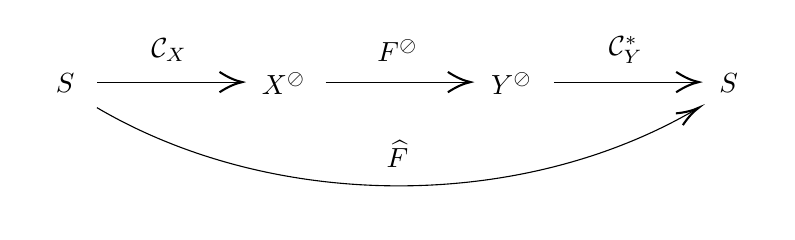
\begin{tikzpicture}[x=0.75pt,y=0.75pt,yscale=-1,xscale=1]
%uncomment if require: \path (0,629); %set diagram left start at 0, and has height of 629

%Straight Lines [id:da560650477859397] 
\draw    (210.17,60.86) -- (278,60.86) ;
\draw [shift={(280,60.86)}, rotate = 180] [color={rgb, 255:red, 0; green, 0; blue, 0 }  ][line width=0.75]    (10.93,-4.9) .. controls (6.95,-2.3) and (3.31,-0.67) .. (0,0) .. controls (3.31,0.67) and (6.95,2.3) .. (10.93,4.9)   ;
%Curve Lines [id:da8170296687430567] 
\draw    (210,73.17) .. controls (295.24,123.25) and (414.47,123.33) .. (498.73,73.92) ;
\draw [shift={(500,73.17)}, rotate = 149.25] [color={rgb, 255:red, 0; green, 0; blue, 0 }  ][line width=0.75]    (10.93,-3.29) .. controls (6.95,-1.4) and (3.31,-0.3) .. (0,0) .. controls (3.31,0.3) and (6.95,1.4) .. (10.93,3.29)   ;
%Straight Lines [id:da24312545548628428] 
\draw    (320.17,60.86) -- (388,60.86) ;
\draw [shift={(390,60.86)}, rotate = 180] [color={rgb, 255:red, 0; green, 0; blue, 0 }  ][line width=0.75]    (10.93,-4.9) .. controls (6.95,-2.3) and (3.31,-0.67) .. (0,0) .. controls (3.31,0.67) and (6.95,2.3) .. (10.93,4.9)   ;
%Straight Lines [id:da8363047188359607] 
\draw    (430.17,60.86) -- (498,60.86) ;
\draw [shift={(500,60.86)}, rotate = 180] [color={rgb, 255:red, 0; green, 0; blue, 0 }  ][line width=0.75]    (10.93,-4.9) .. controls (6.95,-2.3) and (3.31,-0.67) .. (0,0) .. controls (3.31,0.67) and (6.95,2.3) .. (10.93,4.9)   ;

% Text Node
\draw (194.75,61.35) node  [  ] [align=left] {\begin{minipage}[lt]{20.51pt}\setlength\topsep{0pt}
\begin{center}
$S$
\end{center}

\end{minipage}};
% Text Node
\draw (300,61.35) node  [  ] [align=left] {\begin{minipage}[lt]{27.2pt}\setlength\topsep{0pt}
\begin{center}
$X^\oslash$
\end{center}

\end{minipage}};
% Text Node
\draw (409.83,61.35) node  [  ] [align=left] {\begin{minipage}[lt]{26.97pt}\setlength\topsep{0pt}
\begin{center}
$Y^\oslash$
\end{center}

\end{minipage}};
% Text Node
\draw (514.42,61.35) node  [  ] [align=left] {\begin{minipage}[lt]{20.51pt}\setlength\topsep{0pt}
\begin{center}
$S$
\end{center}

\end{minipage}};
% Text Node
\draw (244.83,45.51) node  [  ] [align=left] {\begin{minipage}[lt]{47.83pt}\setlength\topsep{0pt}
\begin{center}
$\mathcal{C}_X$
\end{center}

\end{minipage}};
% Text Node
\draw (354.83,45.51) node  [  ] [align=left] {\begin{minipage}[lt]{47.83pt}\setlength\topsep{0pt}
\begin{center}
$F^\oslash$
\end{center}

\end{minipage}};
% Text Node
\draw (464.83,45.51) node  [  ] [align=left] {\begin{minipage}[lt]{47.83pt}\setlength\topsep{0pt}
\begin{center}
$\mathcal{C}_Y^*$
\end{center}

\end{minipage}};
% Text Node
\draw (354.83,95.51) node  [  ] [align=left] {\begin{minipage}[lt]{47.83pt}\setlength\topsep{0pt}
\begin{center}
$\widehat{F}$
\end{center}

\end{minipage}};


\end{tikzpicture}

\end{figure}
El problema $\widehat{F}$ resuelve el mismo problema que $F$, y es capaz de tratar con entradas erróneas. Basta ver que, si $I\in S$ es una codificación correcta de una entrada $x\in X$ (es decir, $\mathcal{C}_X(I)=x$), entonces es $\widehat{F}(I) = \mathcal{C}_Y^*(F^\oslash(\mathcal{C}_X(I))) = \mathcal{C}_Y^*(F^\oslash(x)) = \mathcal{C}_Y^*(F(x)) = O$, siendo $O$ la codificación de $F(x)$, $O=\mathcal{C}_Y^*(F(x))$. Dada la codificación de la solución $O$, es fácil obtener la solución $F(x) = \mathcal{C}_Y(O)$.

En el caso de que $I \in S$ sea una codificación de entrada incorrecta, será $\widehat{F}(I)=\mathcal{C}_Y^*(F^\oslash(\mathcal{C}_X(I)))=\mathcal{C}_Y^*(F^\oslash(\oslash))=\mathcal{C}_Y^*(\oslash)=\palabra{no}$.
\end{proof}
% ===================+

\pagebreak

\begin{proposicion}\label{prop:ap-cons}
El sistema lógico \normalfont{\textbf{SumaBinariaLógico}} es consistente.
\end{proposicion}
\begin{proof}
Para probar que el sistema es consistente, veremos que todas las reglas de inferencia mapean fórmulas verdaderas a fórmulas verdaderas. En primer lugar, vemos que el axioma \texttt{1=1} es verdadero, pues es cierto que $1=1$.

Ahora, comprobemos cada regla:
$$
    \begin{matrix}
    \text{(R1)} & A\texttt{=}B & \mapsto & \texttt{1+}A\texttt{=}\texttt{1+}B 
    \end{matrix}
$$

En este caso, si $A$ y $B$ son números binarios y asumimos que la fórmula $A\texttt{=}B$ es verdadera, entonces tenemos que $A=B$. Por tanto, la fórmula $\texttt{1+}A\texttt{=1+}B$ es verdadera, ya que es cierto que $1+A=1+B$.
$$
    \begin{matrix}
    \text{(R2)} & A\underline{N}\texttt{+}\underline{N}B & \mapsto & AN\texttt{0}B
    \end{matrix}
$$

El hecho de que las $N$ tengan coincidencias maximales nos lleva a comprobar si dado $N$ un número binario, asumiendo que $N\texttt{+}N$ es verdadera tenemos que $N\texttt{0}$ es verdadera, o lo que es lo mismo, debemos comprobar que $N\texttt{+}N=N\texttt{0}$.

Un número binario $N$ se representa mediante $m$ dígitos, ya sean $0$ o $1$, siendo \linebreak $N=n_{m-1}\:n_{m-2}\:...\:n_1\:n_0$, y se verifica que:
$$N = n_{m-1}\cdot2^{m-1} + n_{m-2}\cdot2^{m-2}+...+n_1\cdot2+n_0$$

Basta ver que:
$$N+N=2N=n_{m-1}\cdot2^{m} + n_{m-2}\cdot2^{m-1}+...+n_1\cdot2^2+n_0\cdot 2$$
y que el número $N+N$ corresponde exactamente a $n_{m-1}\:n_{m-2}\:...\:n_1\:n_0\:0=N\:0$.
$$
    \begin{matrix}
    \text{(R3)} & A\texttt{\underline{1}+}\underline{N\texttt{0}}B & \mapsto & AN\texttt{1}B
    \end{matrix}
$$
De forma análoga a la regla anterior, comprobamos que:
$$1+N\:0=N\:0+1=n_{m-1}\cdot2^{m} + n_{m-2}\cdot2^{m-1}+...+n_1\cdot2^2+n_0\cdot 2+1=N\:1$$
\end{proof}

\begin{proposicion}\label{prop:ap-comp}
El sistema lógico \normalfont{\textbf{SumaBinariaLógico}} es completo.
\end{proposicion}
\begin{proof}
Veremos que toda fórmula verdadera es un teorema. Vemos en primer lugar que toda fórmula verdadera $\phi$ es del tipo
$$\phi=N_1\texttt{+}N_2\texttt{+}...\texttt{+}N_k\texttt{=}M_1\texttt{+}M_2\texttt{+}...\texttt{+}M_l$$
donde cada $N_i, M_j\;\forall i\in\{1, 2, ..., k\}, j\in\{1, 2, ..., l\}$ es un número binario (que verifica la expresión regular $\texttt{1(0|1)}^\texttt{*}$, y de modo que la siguiente fórmula aritmética es cierta:
$$N_1+N_2+...+N_k=M_1+M_2+...+M_l$$
Nuestro objetivo es probar que la fórmula $\phi$ es un teorema. Para ello, vamos a probar que, dado un número binario $n$ que sea compilación maximal de la expresión regular \texttt{1(0|1)*}, éste puede derivarse a partir de la suma de $n$ unos, es decir, debemos probar que:
$$A\underline{n}B\xmapsto{*}A\underbrace{\texttt{1}\texttt{+}\texttt{1}\texttt{+}...\texttt{+}\texttt{1}}_{n)}B$$
Dado que, por ser esto cierto, tenemos que:
$$\psi=\underbrace{\texttt{1}\texttt{+}\texttt{1}\texttt{+}...\texttt{+}\texttt{1}}_{N_1)}\texttt{+}\underbrace{\texttt{1}\texttt{+}\texttt{1}\texttt{+}...\texttt{+}\texttt{1}}_{N_2)}\texttt{+}...\texttt{+}\underbrace{\texttt{1}\texttt{+}\texttt{1}\texttt{+}...\texttt{+}\texttt{1}}_{N_k)}\texttt{=}\underbrace{\texttt{1}\texttt{+}\texttt{1}\texttt{+}...\texttt{+}\texttt{1}}_{M_1)}\texttt{+}\underbrace{\texttt{1}\texttt{+}\texttt{1}\texttt{+}...\texttt{+}\texttt{1}}_{M_2)}\texttt{+}...\texttt{+}\underbrace{\texttt{1}\texttt{+}\texttt{1}\texttt{+}...\texttt{+}\texttt{1}}_{M_l)}\xmapsto{*}\phi$$
Y como tenemos $N_1+N_2+...+N_k$ unos a la izquierda de \texttt{=} y $M_1+M_2+...+M_l$ a la derecha, y es
$$N_1+N_2+...+N_k=M_1+M_2+...+M_l=n$$
tenemos que
$$\psi=\underbrace{\texttt{1}\texttt{+}\texttt{1}\texttt{+}...\texttt{+}\texttt{1}}_{n)}\texttt{=}\underbrace{\texttt{1}\texttt{+}\texttt{1}\texttt{+}...\texttt{+}\texttt{1}}_{n)}$$
pero es claro que podemos obtener $\psi$ aplicando la regla (R1) $n$ veces a partir del axioma $1=1$, luego es
$$\texttt{1=1}\xmapsto{*}\psi=\underbrace{\texttt{1}\texttt{+}\texttt{1}\texttt{+}...\texttt{+}\texttt{1}}_{n)}\texttt{=}\underbrace{\texttt{1}\texttt{+}\texttt{1}\texttt{+}...\texttt{+}\texttt{1}}_{n)}\xmapsto{*}\phi$$
y como $\texttt{1=1}\xmapsto{*}\phi$ y es \texttt{1=1} un axioma, $\phi$ es un teorema.

Probemos que, en efecto, es
$$A\underline{n}B\xmapsto{*}A\underbrace{\texttt{1}\texttt{+}\texttt{1}\texttt{+}...\texttt{+}\texttt{1}}_{n)}B$$

Para ello, primero observemos que, si $m$ es un número binario positivo, entonces puede que sea par o impar.

Si $m$ es impar, entonces puede ser escrito con $k$ dígitos: $m=b_{k-1}\:b_{k-2}\:...\:b_1\:\texttt{1}$. Sea $\varphi$ una fórmula de \textbf{SumaBinariaLógico}, y supongamos que $\varphi$ contiene un \emph{substring} $m$ como compilación maximal de $\texttt{1(0|1)}^\texttt{*}$, es decir, $\phi=A\:\underline{m}\:B$. Entonces, $\varphi$ puede ser derivado de un cierto $\varphi'$, $\varphi'\mapsto\varphi$ mediante la regla (R3), siendo$$\varphi'=A\:\underline{b_{k-1}\:b_{k-2}\:...\:b_1\:\texttt{0}}\:B$$

En caso de que $m$ sea par, es claro que puede expresarse como la suma $p+p$, cierto $p$ un cierto binario positivo. Entonces, si $\varphi$ contiene un \emph{substring} $m$ como compilación maximal de $\texttt{1(0|1)}^\texttt{*}$, $\varphi=A\:\underline{m}\:B$, es $\varphi'\mapsto\varphi$ con $$\varphi'=A\:\underline{p}\texttt{+}\underline{p}\:B$$

Sabiendo esto, cualquier ocurrencia de un entero positivo $m$ en una fórmula de \textbf{SumaBinariaLógico} puede ser reducida a la suma de $m$ unos, es decir, dado $\varphi=A\:\underline{m}\:B$, se tiene que:
$$A\:\underbrace{\texttt{1}\texttt{+}\texttt{1}\texttt{+}...\texttt{+}\texttt{1}}_{m)}\:B\xmapsto{*}\varphi$$
Esto es debido a que todo número natural $m$ puede ser reducido a la suma de $m$ unos aplicando recursivamente las operaciones anteriormente descritas (dividir por $2$ en caso de ser par y restar $1$ en caso de ser impar).
\end{proof}

\begin{proposicion}\label{prop:ap-restr-arr}
El sistema lógico \normalfont{\textbf{SumaBinariaLógicoArreglado}} es completo.
\end{proposicion}
\begin{proof}
Para demostrar esto, usaremos el resultado obtenido en la proposición anterior. Toda fórmula verdadera $\phi$ es del tipo
$$\phi=N_1\texttt{+}N_2\texttt{+}...\texttt{+}N_k\texttt{=}M_1\texttt{+}M_2\texttt{+}...\texttt{+}M_l$$
donde cada $N_i, M_j\;\forall i\in\{1, 2, ..., k\}, j\in\{1, 2, ..., l\}$ es un número binario (que verifica la expresión regular $\texttt{1(0|1)}^\texttt{*}$, y de modo que la siguiente fórmula aritmética es cierta:
$$N_1+N_2+...+N_k\geq M_1+M_2+...+M_l$$
Vamos a llamar a ambas partes con $n$ y $m$:
$$n=N_1+N_2+...+N_k, \;\;\;\;m=M_1+M_2+...+M_l$$
Como $n\geq m$, existe un $p\geq 0$ de modo que $n=m+p$. Ya probamos en la proposición anterior que:
$$\psi=\underbrace{\texttt{1}\texttt{+}\texttt{1}\texttt{+}...\texttt{+}\texttt{1}}_{p)}\texttt{+}\underbrace{\texttt{1}\texttt{+}\texttt{1}\texttt{+}...\texttt{+}\texttt{1}}_{m)}\texttt{=}\underbrace{\texttt{1}\texttt{+}\texttt{1}\texttt{+}...\texttt{+}\texttt{1}}_{m)}\xmapsto{*}\phi$$
Ahora basta ver que:
$$\texttt{1=1}\underset{(1)}{\overset{*}{\longmapsto}}\underbrace{\texttt{1}\texttt{+}\texttt{1}\texttt{+}...\texttt{+}\texttt{1}}_{m)}\texttt{=}\underbrace{\texttt{1}\texttt{+}\texttt{1}\texttt{+}...\texttt{+}\texttt{1}}_{m)}\underset{(2)}{\overset{*}{\longmapsto}}\psi\xmapsto{*}\phi$$
Donde en $(1)$ aplicamos $m$ veces la regla (R1) y en $(2)$ aplicamos $p$ veces la regla (R1b).
\end{proof}

\endinput
